%license:BSD-3-Clause
%copyright-holders:Michele Maione
%============================================================
%
%	MAME Cloud Gaming
%
%============================================================

\chapter{Introduzione}
\label{cap:Introduzione}

Nel 1952 nei laboratori dell'Università di Cambridge come esempio di tesi di dottorato fu creato OXO, la trasposizione del tris come un gioco per computer. Questo di solito è considerato tecnicamente il primo videogioco. Nel 1958 un professore di fisica al Brookhaven National Laboratory creò il gioco Tennis for Two, che aveva il compito di simulare le leggi fisiche che si potevano trovare in una partita di tennis: lo strumento utilizzato era un oscilloscopio.

Nel 1961, sei giovani scienziati del Massachusetts Institute of Technology programmarono, su un PDP-1\footnote{PDP-1: Programmed Data Processor-1, è un computer della Digital Equipment Corporation.} Computer, il primo videogioco adeguatamente progettato: Spacewar!.

Due mesi dopo due ingegneri elettrici N. Bushnell e T. Dabney hanno terminato la loro versione di Spacewar! prodotto su larga scala (1.500 copie), ma il gioco non ebbe comunque un grande successo a causa dell'elevata difficoltà. Bushnell, dopo l'esperimento non particolarmente riuscito, decise però di insistere con i videogiochi, producendoli però in proprio dando vita alla società Atari. Il primo gioco arcade di Atari è stato il primo grande successo del settore: Pong, pubblicato alla fine del 1972, che riproduce approssimativamente la meccanica del ping pong. Atari vendette 19.000 armadi Pong e presto molti imitatori seguirono l'esempio. Alla fine del decennio iniziò l'epoca d'oro dei videogiochi arcade.

\begin{figure}[H]
	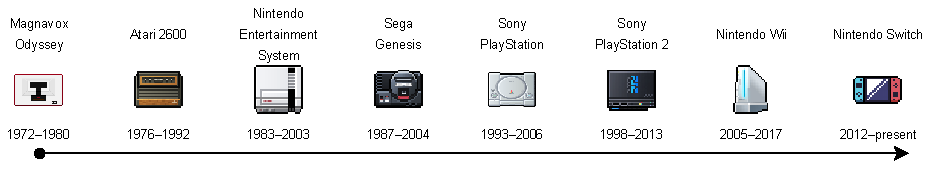
\includegraphics[width=\linewidth]{immagini/consoles_history}
	\caption{Console iconiche, fino alla generazione otto}
	\label{fig:consoles_history}
\end{figure}

Da vent'anni a questa parte l'importanza economica dei videogiochi nei luoghi pubblici è notevolmente diminuita\footnote{Tuttavia, il Giappone, la Cina e la Corea mantengono una forte industria arcade ai giorni nostri.} A favore dei videogiochi per personal computer, console e più recentemente per i dispositivi mobili. Per questo motivo, il termine videogioco arcade viene spesso utilizzato per riferirsi alla generazione di arcade classici\cite{High_Score}.

\section{Cloud gaming}
Il cloud gaming, è un tipo di servizio online che funziona in modo simile al desktop remoto e al video on demand. I videogiochi vengono archiviati ed eseguiti in remoto sull'hardware dedicato di un provider, vengono trasmessi in streaming come un film sul dispositivo di un giocatore tramite client. Il client gestisce gli input del giocatore, che vengono inviati al server ed eseguiti nel gioco.

Questo tipo di approccio offre molti vantaggi, tra cui rendere il gioco più facilmente accessibile senza doverlo scaricare e installarlo localmente, è compatibile con computer e smartphone, anche su smart TV se utilizzato con un gamepad WiFi. Diversi servizi possono offrire alcune funzionalità aggiuntive per sfruttare al meglio questo modello, uno spettatore può unirsi alla sessione di un giocatore e assumere temporaneamente il controllo del gioco, se autorizzato dal giocatore stesso.

Inoltre risolve definitivamente un problema che esiste dai tempi delle cassette compatte e dei floppy disk: la pirateria.

Il rapido sviluppo delle reti a banda larga e il continuo calo dei costi di abbonamento hanno reso questo metodo, oggi, una realtà.

\section{Cloud gaming services}
I primi accenni al cloud gaming per il grande pubblico sono arrivati solo intorno al 2010. Una delle prime piattaforme create per consentire ai giocatori di tutto il mondo di provare l'emozione del gaming in streaming è stata OnLive di OL2. Presentato alla GDC\footnote{GDC: Game Developers Conference, una conferenza annuale per gli sviluppatori di videogiochi.} 2009, poi lanciato sul mercato nel giugno 2010. I giocatori potevano acquistare giochi sulla piattaforma o giocare dal loro Steam\footnote{Steam is un servizio di distribuzione digitale di videogiochi di Valve.} library\footnote{La libreria digitale di videogiochi è la raccolta di videogiochi acquistati da un utente.}.

Nel 2012, Gaikai ha inaugurato il suo servizio di cloud gaming, la società si è concentrata principalmente sull'utilizzo del cloud gaming come forma di pubblicità online per i videogiochi, dove gli utenti avrebbero avuto la possibilità di accedere alle demo dei videogiochi.

OnLive e Gaikai sono stati acquisiti da Sony e le loro risorse sono state utilizzate come base per un servizio di cloud gaming noto come Playstation Now.

Nel 2013, Nvidia ha introdotto GeForce Now, un servizio di cloud gaming integrato nel suo dispositivo Shield TV\footnote{Nvidia Shield TV è un lettore multimediale digitale basato su Android TV prodotto da Nvidia.} Dispositivo. Nel 2017, la società ha iniziato a espandere il proprio servizio su PC, incluso il supporto per l'importazione della libreria Steam di un utente.

Nel maggio 2018, Electronic Arts ha acquisito alcune risorse di cloud gaming da GameFly. EA\footnote{EA: Electronic Arts.} Ha annunciato Project Atlas, un progetto che esplorava l'integrazione di intelligenza artificiale e apprendimento automatico, rendendo la piattaforma dinamica, social e multipiattaforma.

Microsoft all'E3\footnote{E3: Electronic Entertainment Expo, un evento commerciale per l'industria dei videogiochi.} Il 2018 ha anticipato il suo servizio Xbox Cloud Gaming.

Alla GDC 2019, Google ha annunciato ufficialmente il suo servizio di cloud gaming Stadia, in uscita per novembre dello stesso anno.

A settembre 2020, un nuovo servizio chiamato Luna è stato annunciato da Amazon\cite{Cloud_gaming_history}.

\subsubsection{Apple's controversy}
Apple aveva cercato di bloccare le app di cloud gaming sul suo servizio a metà del 2020 su piattaforma iOS, ma a settembre 2020 ha modificato le sue regole che consentivano il cloud gaming con le restrizioni che i giochi offerti nel servizio devono essere scaricati direttamente dall'App Store, non da un'app all-in-one. I produttori di app sono autorizzati a rilasciare una cosiddetta "app catalogo" che si collega ad altri giochi nel servizio, ma ogni gioco dovrà essere una singola app e tutti i giochi e i negozi devono offrire l'acquisto in-app utilizzando l'app Apple. sistema di elaborazione dei pagamenti, in base al quale Apple di solito prende il 30\% delle entrate\cite{Apple_controversy}.

\subsubsection{Cloud gaming market}
Secondo la ricerca di Newzoo sull'industria dei videogiochi, nel 2020 sono stati generati quasi \$585 milioni di entrate dal mercato del cloud gaming ed è destinato a crescere notevolmente fino a \$4,8 miliardi entro il 2023. Oltre a ciò, la proiezione attuale suggerisce addirittura crescita maggiore. Per questo sono entrate nel mercato anche aziende che non sono produttori di videogiochi, come Google e Amazon.

\begin{figure}[H]
	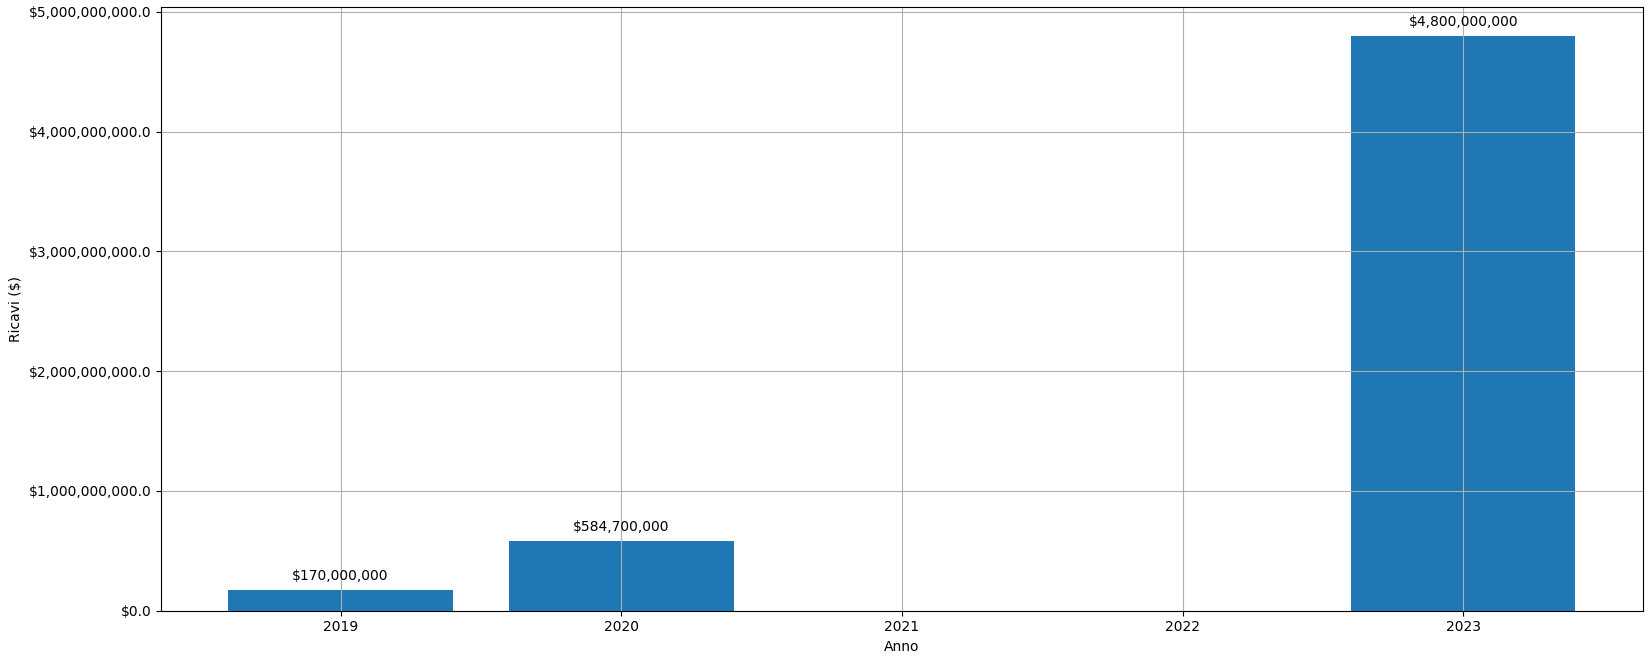
\includegraphics[width=\linewidth]{immagini/Newzoo_Cloud_Gaming_Revenues}
	\caption{Previsioni sulla capitalizzazione di mercato globale del cloud gaming in dollari americani. Fonte: newzoo.com/global-cloud-gaming-report}
	\label{fig:Newzoo_Cloud_Gaming_Revenues_Sept_2020}
\end{figure}

Vediamo l'attuale panorama del cloud gaming.

\subsection{Utomik}
La piattaforma Utomik è stata lanciata commercialmente nel 2008 e da allora è in servizio. I giochi per essere riprodotti in un browser richiedono il plug-in proprietario Utomik Player. La piattaforma offre un SDK\footnote{SDK: kit di sviluppo software, una raccolta di strumenti di sviluppo software.}, Plug-in e servizio online per creare, avviare, mantenere e monitorare i giochi \cite{Utomik}.

\subsection{Microsoft - Xbox Cloud Gaming}
Microsoft ha anticipato il servizio all'E3 2018. Il servizio è disponibile per gli abbonati a Xbox Game Pass Ultimate dal 15 settembre 2020. La piattaforma offre la libreria esistente di giochi Xbox e aggiunge nuovi giochi da Xbox Series X. Il servizio è progettato per funzionare con i telefoni (attualmente solo Android), con controlli touchscreen o controller Xbox tramite Bluetooth\cite{Xbox_Game_Pass_cloud_gaming}.

\subsection{Project Atlas}
A maggio 2018 Electronic Arts ha svelato la sua piattaforma di gioco nativa per il cloud chiamata Project Atlas, che mira a rendere disponibili numerosi titoli giocabili attraverso i server dell'azienda ea fornire un'esperienza di gioco mai provata prima grazie al supporto dell'intelligenza artificiale. La piattaforma intende offrire un'esperienza di cloud gaming composta da universi realmente viventi, che cambiano con il passare del tempo, con l'interazione con altri giocatori e sotto l'influenza del mondo esterno. In questi processi, il supporto dell'intelligenza artificiale e l'apprendimento delle abitudini e delle preferenze dei giocatori giocherebbero un ruolo fondamentale. Offre anche un client di gioco dinamico, che consente agli utenti di riprodurre in streaming un titolo mentre attendono il completamento del download sul disco di archiviazione del proprio dispositivo\cite{Project_Atlas}.

\subsection{Nvidia - GeForce Now}
GeForce Now è il servizio di cloud gaming di Nvidia lanciato in beta a gennaio 2017 e ufficialmente a febbraio 2020. GeForce Now consente agli utenti di accedere da remoto (tramite streaming) a un computer virtuale, dove possono installare i giochi acquistati su Steam, Ubisoft Connect\footnote{Ubisoft Connect è un servizio di distribuzione digitale, gestione dei diritti digitali, multiplayer e comunicazione sviluppato da Ubisoft.} O Epic Games Store\footnote{Epic Games Store è un negozio di videogiochi digitali gestito da Epic Games.}. Il servizio può essere utilizzato su Windows, macOS, iOS, Android o Nvidia Shield TV\cite{GeForce_Now}.

\subsection{Sony - PlayStation Now}
PlayStation Now è un servizio di abbonamento al cloud gaming basato sulla tecnologia cloud di Gaikai e Microsoft Azure. È stato presentato durante il CES\footnote{CES: Consumer Electronics Show, un evento annuale che ospita presentazioni di nuovi prodotti e tecnologie nel settore dell'elettronica di consumo.} 2014. È disponibile da gennaio 2015 in Nord America, da settembre in Giappone e Regno Unito . Il servizio ha iniziato ad operare in Europa gradualmente da agosto 2017 a marzo 2019. Il servizio consente all'utente di giocare ai titoli PlayStation (dal catalogo giochi di PS2, PS3 e PS4) su PS4, PS5 e Windows\cite{PlayStation_Now}.

\subsection{Google - Stadia}
Stadia è una piattaforma di cloud gaming rilasciata a novembre 2019, ma è disponibile solo in Europa e negli Stati Uniti. Sulla piattaforma l'utente può acquistare giochi o iscriversi al servizio per accedere al catalogo giochi.

Google ha creato il controller Stadia che si connette tramite WiFi direttamente al servizio e rende possibile giocare su una TV (installando l'app o utilizzando un Chromecast \ footnote {Google Chromecast is digital media player for Internet-streamed audiovisual content}). Puoi giocare con mouse e tastiera o controller utilizzando il browser Chrome su qualsiasi PC. È disponibile un'app mobile che supporta i controlli touch screen e i gamepad Bluetooth.

La piattaforma offre alcune funzionalità interessanti come: condividere il gameplay tramite un live streaming su YouTube; Crowd Play che consente agli spettatori di unirsi ai giochi multiplayer che stanno guardando; Stream Connect che consente all'utente di condividere la schermata di gioco con altri giocatori nello stesso gioco; Condivisione dello stato che consente ai giocatori di condividere il proprio stato di salvataggio\cite{Google_Stadia}.

\subsection{Amazon - Luna}
Luna è stata annunciata il 24 settembre 2020, con "accesso anticipato" disponibile per gli abbonati su invito a partire dal 20 ottobre 2020. Amazon Luna avrà 100 giochi diversi al lancio e sarà alimentato da AWS. Luna avrà l'integrazione con Twitch. Amazon ha stretto una partnership con Ubisoft per creare un canale di gioco (con costi aggiuntivi) esclusivo di Luna, che darà agli abbonati di Luna l'accesso ai titoli di Ubisoft lo stesso giorno in cui vengono rilasciati.\cite{Amazon_Luna}.

\subsection{RemoteMyApp - Vortex}
Il servizio è stato lanciato a novembre 2018. Il servizio è disponibile per Android, Windows e macOS, offre tre piani mensili (\$12, \$23 e \$33) che consentono all'utente di giocare per un massimo di 140 ore al mese e il catalogo è composto da 170 giochi. Sfortunatamente, alcuni giochi possono essere riprodotti solo acquistando la licenza del gioco\cite{RemoteMyApp_Vortex}.

\subsection{Playkey}
Una menzione speciale va fatta alla società Playkey, che ha realizzato una piattaforma di cloud gaming distribuita. I giocatori non si connettono a un server per ricevere lo streaming del gioco, ma al computer di un minatore, su cui viene eseguito il gioco. Non ci sono server potenti, perché ci sono computer distribuiti in tutto il mondo che fungono da server, i minatori guadagnano \$10 al giorno. I giocatori possono giocare solo dalla loro libreria di giochi personale\cite{Playkey}.

\section{Proposed system}
Una caratteristica fondamentale del sistema è l'usabilità e per questo, lato client, il browser web è stata la scelta più ovvia.
Esistono alcune tecnologie di streaming per i browser web: WebSocket, HLS, DASH e WebRTC\cite{Audio_and_video_delivery}.

WebSocket è un protocollo di comunicazione che fornisce canali di comunicazione full-duplex su una singola connessione TCP, con una latenza inferiore rispetto a HLS e DASH.

HTTP Live Streaming (HLS) è il protocollo di streaming ad alta latenza più popolare su HTTP per video on demand (video preregistrato) sviluppato da Apple.

Dynamic Adaptive Streaming over HTTP (DASH) è una tecnica di streaming bit rate adattiva di Moving Picture Experts Group (MPEG), che consente lo streaming di alta qualità di contenuti multimediali su HTTP.

Web Real-Time Communication (WebRTC) è un progetto per la comunicazione in tempo reale basato sul protocollo SRTP (Secure Real-time Transport Protocol). Pertanto, per ottenere il flusso SRTP nel browser è necessario un server WebRTC\cite{High_Performance_Browser_Networking}.

\begin{figure}[H]
	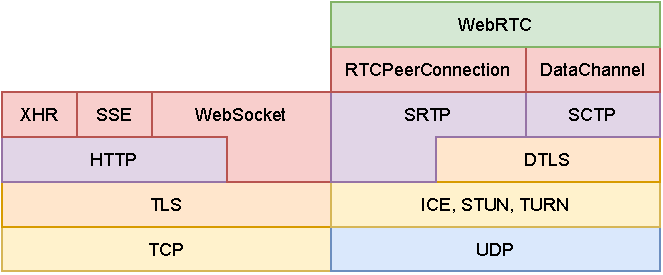
\includegraphics[width=\linewidth]{immagini/webprotocols}
	\caption{API, protocolli e servizi di rete del browser di alto livello}
	\label{fig:webprotocols}
\end{figure}

Questo progetto è pensato per essere utilizzato in stand di retro-gaming in eventi commerciali per l'industria IT e dei videogiochi, verrà eseguito su una rete locale e gli utenti sono connessi tramite WiFi, quindi la differenza di velocità tra TCP e UDP diventa trascurabile, quindi il la scelta è ricaduta su WebSocket perché è un protocollo di comunicazione standardizzato dal 2011, è pienamente supportato da tutti i browser moderni, è semplice e non richiede l'utilizzo di protocolli aggiuntivi o configurazioni complesse a differenza di WebRTC.

\begin{figure}[H]
	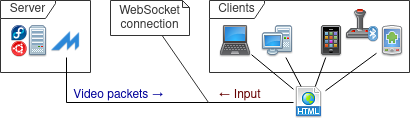
\includegraphics[width=\linewidth]{immagini/proposed_system}
	\caption{Panoramica del sistema}
	\label{fig:proposed_system}
\end{figure}

Il sistema è costituito da un server di gioco, che può essere Linux, Windows o macOS, che esegue MAME e una pagina HTML5 che funge da front-end.

Il programma sta ascoltando una connessione WebSocket che include parametri, come il nome del gioco. Una volta stabilita la connessione, il server invia informazioni sulla dimensione e le proporzioni del video e avvia il gioco. Il rendering e il missaggio audio del gioco vengono generati tramite SDL\footnote{SDL: Simple DirectMedia Layer, una libreria di sviluppo software multipiattaforma progettata per fornire un livello di astrazione hardware per componenti hardware multimediali del computer.}, Codificati e pacchettizzati in MPEG-TS\footnote{MPEG-TS: MPEG transport stream, è un formato contenitore digitale standard per la trasmissione e l'archiviazione di audio e video.} tramite FFmpeg\footnote{FFmpeg è una vasta suite open source di librerie e programmi per la gestione di video, audio, e altri file multimediali e stream.}. I pacchetti vengono inviati tramite WebSocket al client.

Lato client vari script si occuperanno di decodificare i dati audio / video ricevuti, catturare e inviare l'input dell'utente, sia dalla tastiera che dal gamepad, al server tramite WebSocket.